%%%%%%%%%%%%%%%%%%%%%%%%%%%%%%%%%%%%%%%%%%%%%%%%%%%
%% P3: Phenomenology of Particle Physics                         
%%
%% Author:  André Rubbia                   		 
%%
%% Figure 14.3 Schematic of the three decoupled periodic motions in a Penning trap.
%%
%% This work is licensed under the Creative Commons Attribution 4.0 International License. 
%% To view a copy of this license, visit http://creativecommons.org/licenses/by/4.0/ or 
%% send a letter to Creative Commons, PO Box 1866, Mountain View, CA 94042, USA.
%%
%%%%%%%%%%%%%%%%%%%%%%%%%%%%%%%%%%%%%%%%%%%%%%%%%%%

\documentclass[a4paper,10pt]{article}

\usepackage[T1]{fontenc}
\usepackage[utf8]{inputenc}
\usepackage{lmodern}
\usepackage[labelfont=bf]{caption}
\usepackage{upgreek}

\usepackage{tikz}
\usepackage{pgfplots}
\pgfplotsset{compat=1.17}
\usepgfplotslibrary{ternary}
\usepgfplotslibrary{fillbetween}
\usepgfplotslibrary{external}

\usepackage{braket}

\def\d{\mathrm{d}}

\pgfkeys{/pgf/number format/.cd,1000 sep={}}

\begin{document}

%%%%%%%%%%%%%%%%% FIGURE %%%%%%%%%%%%%%%%%%%%%%%%%%%%%%%%%%
\begin{figure}[htb]
\begin{center}
\vspace{-0.5cm}
{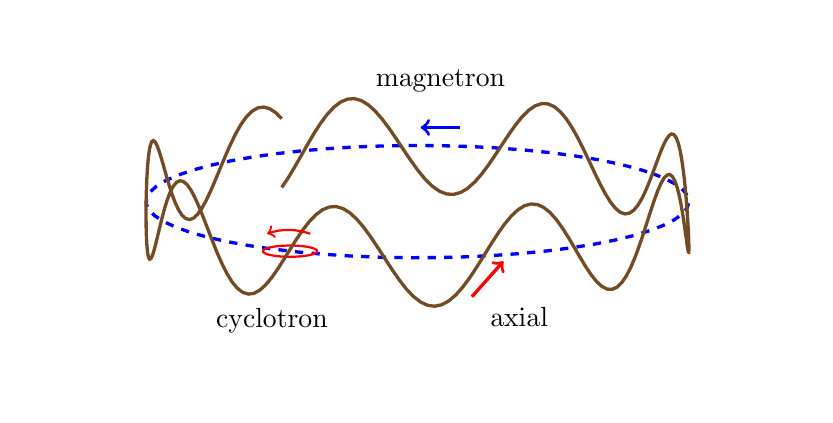
\begin{tikzpicture}
\begin{axis}[view={60}{30},
width=11cm,
height=6cm,
xticklabel=\empty,
yticklabel=\empty,
zticklabel=\empty,
zmin=-1, zmax = 1,
axis line style={draw=none},
tick style={draw=none}]
\addplot3+ [ domain=0:2*pi,
samples = 60,
samples y=0, no marks, very thick, dashed
] (
{sin(deg(x))}, {cos(deg(x))}, {0 }
);
\addplot3+ [ domain=0:2*pi,
samples = 60,
samples y=0, no marks, thick
] (
{0.1*sin(deg(x))+sin(148)}, {0.1*cos(deg(x))+cos(148)}, {0 }
);
\addplot3+ [ domain=-0.5*pi:1.5*pi,
samples = 240,
samples y=0, no marks, very thick
] (
{sin(deg(x))}, {cos(deg(x))}, {0.5*sin(deg(x*8.5)) }
);
\end{axis}
\draw[blue, very thick, <-] (4.75,3.15) -- (5.25,3.15);
\node at (5,3.75) {magnetron};
\draw[red, very thick, ->] (5.4,1) -- +(0.4,0.45);
\node at (6,0.75) {axial};
\draw[thick,red,<-] (2.8,1.8) arc(110:70:0.8);
\node at (2.86,0.7) {cyclotron};
\end{tikzpicture}
}
\vspace{-0.5cm}
\caption{Schematic of the three decoupled periodic motions in a Penning trap called magnetron (dashed),
axial (wavy), and cyclotron (fast circular).}
\end{center}
\end{figure}
%%%%%%%%%%%%%%%%% END FIGURE %%%%%%%%%%%%%%%%%%%%%%%%%%%%%%
%

\end{document}
